\documentclass[a4paper, 12pt]{extarticle}

\usepackage[french, english]{babel}
\usepackage[utf8]{inputenc}
\usepackage[T1]{fontenc}
\usepackage{graphicx}
\usepackage{multirow}
\usepackage{tikz}

\usepackage{fancyhdr, lastpage}
\pagestyle{fancy}
\fancyfoot[C]{{\thepage}/\pageref{LastPage}}

% \usepackage{fontspec}
% \setmainfont{Times New Roman}
\usepackage{geometry}
\geometry{a4paper,
    total={170mm,257mm},
    left=20mm,
    top=7mm,
 }

% !TeX root = ./kernel/esayRattra.tex

\newcommand{\courseCode}{--}
\newcommand{\courseTitle}{Réseaux intelligents et réseaux industriels}
\newcommand{\examDate}{12 février 2020}
\newcommand{\examType}{RATTRAPAGE}
\newcommand{\teacher}{M. LIEDJI WENKACK Dagobert}
\newcommand{\semester}{1}
\newcommand{\academicYear}{2020-2021}
\newcommand{\timeAllowed}{2 Heures 00 Minutes}
\newcommand{\totalMarks}{20}
\newcommand{\MarksOne}{\scriptsize{(4 points)}}
\newcommand{\MarksTwo}{\scriptsize{(11 points)}}
\newcommand{\MarksThree}{\scriptsize{(5 points)}}
\newcommand{\classLevel}{Master 2 RTS}
\newcommand{\docs}{Aucun}
\begin{document}

\begin{center}
    \begin{tabular}{ccc}
        \textbf{REPUBLIC OF CAMEROON }              & \multirow{7}{*}{\resizebox{3cm}{4cm}{
\includegraphics{../figs/ic_logo.jpg}}} & \textbf{REPUBLIQUE DU CAMEROUN}          \\
        \scriptsize \textbf{PEACE-WORK-FATHERLAND } &                                                                              & \scriptsize \textbf{PAIX-TRAVAIL-PATRIE} \\
        {\small **********}                         &                                                                              & {\small **********}                      \\
        \textbf{UNIVERSITY OF DSCHANG}              &                                                                              & \textbf{UNIVERSITE DE DSCHANG}           \\
        {\small **********}                         &                                                                              & {\small **********}                      \\
        \textbf{FACULTY OF SCIENCE}                 &                                                                              & \textbf{FACULTE DES SCIENCE}             \\
        {\small **********}                         &                                                                              & {\small **********}                      \\
        \textbf{Deparment of physics}               &                                                                              & \textbf{Département de Physique}         \\
    \end{tabular}
\end{center}
% \vspace{0.2cm}
{\centering \rule{\linewidth}{0.03cm}}

\begin{center}
    \textbf{\courseTitle (\courseCode)}\\
    \textbf{Correction}
\end{center}
\vspace{-0.5cm}
\begin{center}
    \scriptsize
    \begin{tabular*}{\textwidth}{l @{\extracolsep{\fill}} l}
        \textbf{Niveau:} \classLevel & \textbf{Durée:} \timeAllowed\\
        \textbf{Année Académique:} \academicYear & \textbf{Session:} \examType\\
        \textbf{Semestre:} \semester & \textbf{Date:} \examDate\\
        \textbf{Document autorisés:} \docs & \textbf{Enseignant:} \teacher\\
    \end{tabular*}
\end{center}
\vspace{-0.5cm}
{\centering \rule{\textwidth}{0.02cm}}

% !TeX root = ./kernel/easyRattraSolution.tex
% !TeX root = ./kernel/EasySolution.tex

\section*{Solution du test de connaissances \MarksOne}
\begin{enumerate}
    \item Définition des termes:
          \begin{itemize}
              \item{\textbf{Les réseaux intelligents} sont des réseaux matériels de distributions de fluides (électricité, eau, gaz, pétrole...), \emph{et/ou d'information (télécommunications)} qui ont été « augmentés » (rendus intelligents) par des systèmes informatiques, capteurs, interfaces informatiques et électromécaniques leur donnant des capacités d'échange bidirectionnel et parfois une certaine capacité d'autonomie en matières de calcul et gestion de flux et traitement d'information.}
              \item \textbf{Capteurs, signal, échantillonnage et actionneurs}
                    \begin{itemize}
                        \item Un capteur est un dispositif transformant l'état d'une grandeur physique observée en une grandeur utilisable appelé signal.
                        \item Un signal est formellement définit comme une fonction d'une ou plusieurs variables qui transmettent des informations sur la nature d'un phénomène physique.
                        \item L'échantillonnage est la première étape dans la numérisation d'un signal et consiste à convertir le signal du message en une séquence de nombres, chaque nombre représentant l'amplitude du signal du message à un instant discrét donné.
                        \item Actionneurs: dispositifs physiques qui déclenchent une action précise lorsqu'ils reçoivent un signal externe.
                    \end{itemize}
          \end{itemize}
    \item Donner la signification des protocoles d'échange de données, de et de sécurité des réseaux intélligents suivants:
          \begin{enumerate}
              \item HTTP:  Hypertext Transfer Protocol
              \item M2M : Machine to machine communication Protocol
              \item CoAP: Constrained Application Protocol
              \item MQTT: Message Queuing Telemetry Transport
              \item SSL: Secure Socket Layer
              \item TLS: Transport Layer Security
              \item DTLS: Datagram Transport Layer Security
          \end{enumerate}
    \item Donner et définissez deux autres protocoles des réseaux intelligents de votre choix.
          \begin{itemize}
              \item DDS: Data-Distribution Service
              \item AMQP : Advanced Message Queuing Protocol
              \item XMPP: Extensible Messaging and Presence Protocol
          \end{itemize}
\end{enumerate}


% !TeX root = ./kernel/easyRattraSolution.tex
% !TeX root = ./kernel/EasySolution.tex
\section*{Solution de l'exercice 2 \MarksThree}

\begin{enumerate}
    \item Donnez trois systèmes d'exploitations utilisés dans la mise en place des réseaux intelligents.
          \begin{itemize}
              \def\mydata{TinyOS, RIOT, Contiki, Mantis OS, Nano RK, LiteOS, FreeRTOS, Apache Mynewt,
                  Zephyr OS, Ubuntu Core 16, ARM mbed, Yocto, Raspbian, Andriod Things, Huawei
                  LightOS, Snappy, etc.}
              \foreach \x in \mydata{\item \x}
          \end{itemize}
    \item Citez deux (02) outils logiciels et quatre (04) outils matériels utilisés
          \begin{itemize}
              \item Arduino framework, FreeRTOS
              \item Arduino, esp8266, STM32, Raspberry pi
          \end{itemize}
    \item Citez quatre (04) applications des réseaux intelligents.
          \begin{itemize}
              \item Automobile
              \item Smart grids
              \item Agriculture
              \item Transport
              \item Smart city
          \end{itemize}
    \item Donnez quatre (04) des risques encourus par une organisation ayant un réseaux intelligent mal sécurisé ?
          \begin{itemize}
              \item Prendre le contrôle des appareils multifonctions pour perturber mali-
                    cieusement l’accès à Internet (par exemple, l’attaque du réseau de zom-
                    bies)
              \item Accès à des microphones à distance sur les appareils reseaux intelligent
                    pour écouter des conversations sensibles
              \item Prendre le contrôle des caractéristiques d’une voiture (par exemple,
                    altération des freins d’un véhicule)
              \item L’accès à des données sensibles ou à des informations personnelles (par
                    exemple, les noms des clients et les cartes de crédit) par l’intermédiaire
                    de dispositifs reseaux intelligent non sécurisés qui sont connectés aux
                    réseaux des entreprises
          \end{itemize}
    \item Donnez quatre (04) tâches a éffectuer afin de sécuriser les dispositifs des réseaux intelligents ?
          \begin{itemize}
              \item Modification des mots de passe par défaut sur les appareils reseaux
                    intelligent. Si les règles relatives aux mots de passe le permettent,
                    utilisez des phrases de passe, plutôt que des mots de passe, sur tous les
                    appareils reseaux intelligent sur le lieu de travail.
              \item tiliser l’authentification à deux facteurs pour les dispositifs ou les
                    applications afin d’ajouter une couche de sécurité supplémentaire.
              \item S’assurer que les données générées par les éléments de l’reseaux intelli-
                    gent sont cryptées.
              \item Désactivation de toute fonctionnalité de connexion automatique (par
                    exemple, plug and play)
          \end{itemize}
    \item Donner deux (02) avantages des réseaux intelligents.
          \begin{itemize}
              \item Réduction des coûts (optimisation des équipements, gestion de tournées, économie d’énergie)
              \item Optimisation des processus métiers (détection des pannes, des lieux d’intervention facilitée, maintenance industrielle optimisée.)
              \item Création de nouveaux services (être plus proche des clients finaux, accèder en temps réel aux besoins, intervenir au moment opportun.)
          \end{itemize}
    \item Identifiez et classifier les cartes de la figure \ref{fig:carte} en carte à microcontrôleurs ou en carte à microprocesseur.
          \begin{itemize}
              \item Cartes à microprocesseur : raspberry pi 3 model B et raspberry pi zéro.
              \item Carte à microcontrolleur: Arduino Uno.
          \end{itemize}
\end{enumerate}

\begin{figure}[!ht]
    \centering
    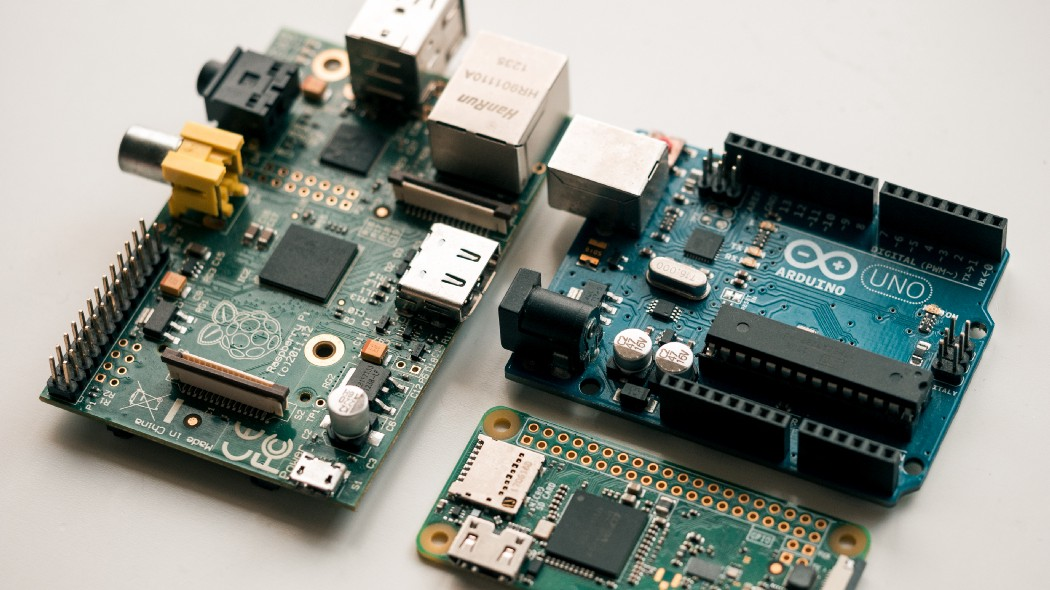
\includegraphics[scale=0.25]{../../figs/hardware_devices.jpg}
    \caption{Quelques cartes pour réseaux intélligents.\label{fig:carte}}
\end{figure}
% !TeX root = ./kernel/easyRattraSolution.tex

% !TeX root = ./kernel/EasySolution.tex
\section*{Solution de l'exercice 1 \MarksTwo}

\begin{enumerate}
      \item Décrivez brièvement le fonctionnement d'un réseaux intélligent.
            \begin{itemize}
                  \item Les réseaux intelligents fonctionnent principalement avec des capteurs et objets connectés placés dans / sur des infrastructures physiques. Ces capteurs vont alors émettre des données qui vont remonter à l’aide d’un réseau sans fil sur des plateformes de réseaux intelligents. Elles pourront être ainsi analysées et enrichies pour en tirer le meilleur profit. Ces plateformes de data management et de data visualisation sont les nouvelles solutions intelligentes permettant aux territoires, entreprises ou même usagers d’analyser les données et d’en tirer des conclusions pour pouvoir adapter pratiques et comportements.
            \end{itemize}
      \item Donner la représentation de l’architecture d’un projet réseau intelligent.
            \begin{itemize}
                  \item Voir la figure \ref{fig:arch}
            \end{itemize}
            \begin{figure}[!ht]
                  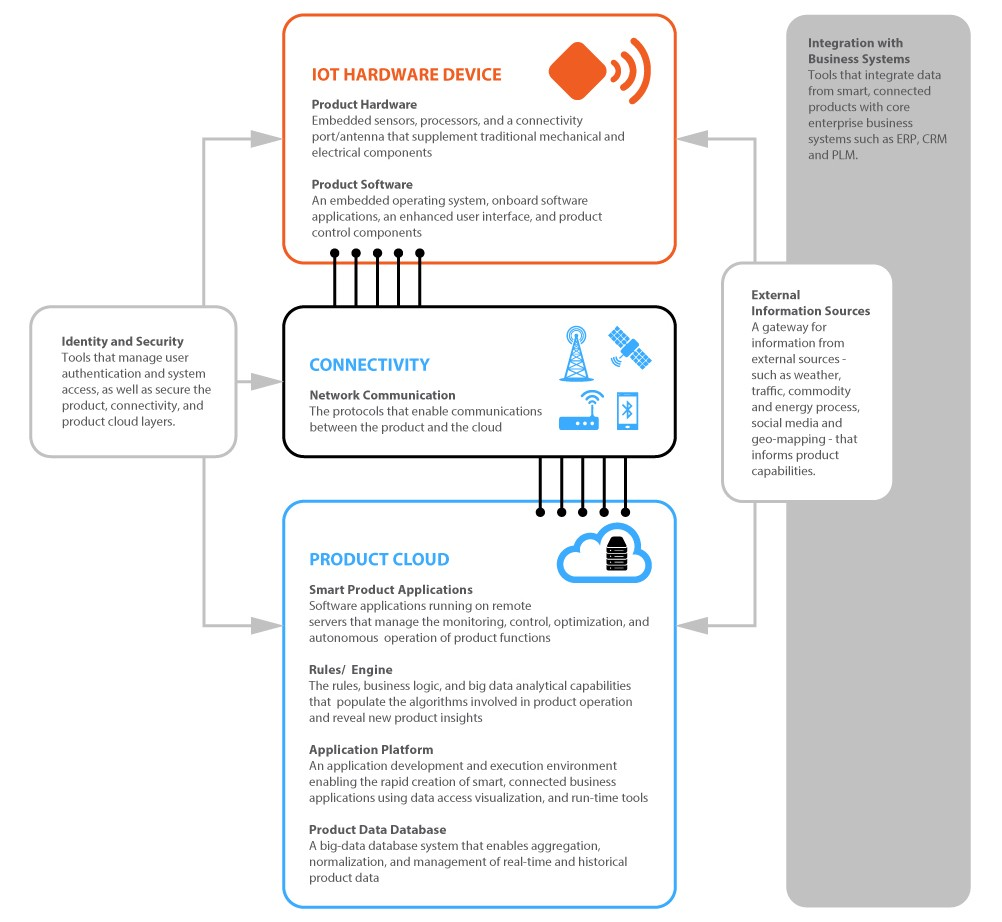
\includegraphics[trim={1cm, 0cm, 0cm, 0cm}, width=18cm, clip]{../../figs/iot_arch.jpeg}
                  \caption{Représentation de l'architecture d'un projet de réseau intélligent.}
                  \label{fig:arch}
            \end{figure}
      \item Citez en donnant les fonctions de chaque couches de l'architecture des réseaux intélligents.
            \begin{itemize}
                  \item  Composant hardware : le dispositif physique qui interagit avec l’environnement.
                  \item Connectivité : le lien entre votre appareil et le cloud
                  \item produits du cloud : serveurs qui prennent des données, les traitent, les
                        stockent dans des bases de données, donnent des commandes, effectuent
                        des analyses, servent les données de manière utile à tous les différents
                        acteurs.
            \end{itemize}
      \item Citez 05 (cinq) protocoles des réseaux intélligents.
            \begin{itemize}
                  \item Bluetooth
                  \item LoRaWAN
                  \item RFID/NFC
                  \item WiFi
                  \item 6LoWPAN
            \end{itemize}
      \item Quelle est la couche de l'architecture des réseaux intélligents qui interagit directement avec les processus industriels ?
            \begin{itemize}
                  \item Couche Hardware ou matériel.
                  \item Cette interaction se fait à travers de capteurs et actionneurs.
            \end{itemize}
      \item Donnez la différence entre un réseaux dit "non intélligent" et un réseaux intélligent.
            \begin{itemize}
                  \item{Les réseaux intelligents sont des réseaux matériels de distributions de fluides (électricité, eau, gaz, pétrole...), et/ou d'information (télécommunications) qui ont été « augmentés » (rendus intelligents) par des systèmes informatiques, capteurs, interfaces informatiques et électromécaniques leur donnant des capacités d'échange bidirectionnel et parfois une certaine capacité d'autonomie en matières de calcul et gestion de flux et traitement d'information.}
            \end{itemize}
\end{enumerate}
La figure \ref{fig:iiot} montre le chef mécanicien vérifiant et contrôlant des robots robots d'automatisation des bras dans l'industrie intelligente d'usine sur le logiciel de système de surveillance en temps réel.

\begin{enumerate}
    \item Donnez trois (03) protocoles réseaux adaptés dans la mise en place de ce réseau intélligent industriel (voir figure \ref{fig:iiot}).
          \begin{itemize}
              \item Wifi
              \item LoRaWan
              \item GSM/GPRS
          \end{itemize}
    \item Donnez les élements de chaque couche de l'architecture d'un réseau intélligent se trouvant sur la figure \ref{fig:iiot}.
          \begin{itemize}
              \item Couche Hardware: représentée par les robots et capteur connectés au serveur central.
              \item Couche de connectivité: représentée par les protocoles réseaux (LoRaWan, Wifi, GSM/GPRS, etc.)
              \item Couche du cloud: représentée par l'ordinateur central du mécanicien chef.
          \end{itemize}
    \item Donnez deux (02) avantages de ce réseau sur une industrie.
          \begin{enumerate}
              \item Une augmentation de production
              \item Favorise une meilleure collaboration entre les employés.
              \item Facilite l'échange et le partage d’information au sein de l'industrie.
              \item Garantie une sécurité des employés car le contrôle se faits à distance.
          \end{enumerate}
    \item Donnez deux (03) tâches à éffectuer afin d'éviter l'attaque des robots réseau sur les employés de cette l'industrie.
          \begin{enumerate}
              \item Rendre le matériel (robots, capteurs, etc.) inviolable.
              \item Utilisation d'une l’authentification forte.
              \item Utiliser un cryptage fort et des protocoles sécurisés.
              \item Diviser les réseaux en segments.
          \end{enumerate}
\end{enumerate}

\begin{figure}[!ht]
    \centering
    
\includegraphics[scale=1.4]{../../figs/industrial_inttelings.jpg}
    \caption{Le chef mécanicien vérifie et contrôle des robots, robots d'automatisation à bras dans l'industrie intelligente d'usine sur le logiciel de système de surveillance en temps réel.}
    \label{fig:iiot}
\end{figure}


\end{document}